\documentclass[pdflatex,sn-basic,Numbered]{sn-jnl}

\usepackage{graphicx}
\usepackage{multirow}
\usepackage{amsmath,amssymb,amsfonts}
\usepackage{xcolor}
\usepackage{booktabs}
\usepackage{url}
\usepackage{tabularx}
\usepackage{array}
\usepackage{geometry}
\geometry{top=2.6cm, bottom=2.6cm, footskip=1cm}

\graphicspath{{figures/}{../figures/}}

\setcounter{topnumber}{4}
\setcounter{bottomnumber}{2}
\setcounter{totalnumber}{6}
\renewcommand{\topfraction}{0.95}
\renewcommand{\bottomfraction}{0.85}
\renewcommand{\textfraction}{0.05}
\renewcommand{\floatpagefraction}{0.80}
\setlength{\textfloatsep}{8pt plus 2pt minus 2pt}
\setlength{\floatsep}{8pt plus 2pt minus 2pt}
\setlength{\intextsep}{8pt plus 2pt minus 2pt}
\setlength{\tabcolsep}{5pt}
\renewcommand{\arraystretch}{1.12}
\newcolumntype{Y}{>{\raggedright\arraybackslash}X}
\linespread{1.05}

\raggedbottom

\begin{document}
\title[ACP-Gini: Path-dependent Correlation Penalization]{ACP-Gini: Path-dependent Correlation Penalization for Decision Tree Induction}

\author[1]{\fnm{Khang} \sur{Lam Huynh}}\email{khanglhse200666@fpt.edu.vn}

\author[1]{\fnm{Dat} \sur{Phan Tuan}}\email{ptundatwork@gmail.com}

\author[1]{\fnm{Nhan} \sur{Nguyen Trong}}\email{hi.gesar@gmail.com}

\author[1]{\fnm{Huy} \sur{Nguyen Xuan}}\email{huynx23@fe.edu.vn}

\affil*[1]{\orgdiv{Artificial Intelligence}, \orgname{FPT University}, \orgaddress{\city{Ho Chi Minh City}, \country{Vietnam}}}

\abstract{
Decision trees avoid coefficient estimation under multicollinearity, yet greedy induction still splits on interchangeable members of correlated predictor groups, which yields redundant feature sets and disperses importance over proxies. We introduce ACP-Gini, a single-tree splitting criterion that multiplies each candidate's raw Gini gain by a product of correlation penalties against the distinct features already used on the root-to-node path. It reduces to CART at $\alpha=0$ and keeps raw gain for stopping. On twelve binary-classification data sets evaluated over 15 held-out folds, four of them strongly collinear, ACP-Gini lowered bootstrap importance-weighted redundancy in every data set (median reduction 12.5\%, range 0.9\% to 32.3\%; all Holm-adjusted $p\le0.0013$), and under Spearman and mutual-information measures that the penalty does not use. Against VIF pruning it was significantly better on two of the four strongly collinear sets (Parkinsons, Ozone) and worse on two (WDBC, Landsat), where VIF discarded most features. No accuracy change was significant, but the 95\% intervals do not exclude losses of several points (up to 5.5 on Parkinsons, 9.0 with nested tuning). Used-feature stability fell on eleven data sets and importance-rank stability fell significantly on four while rising on two. A tree-global correlation penalty gave an equal or slightly larger average reduction; only in a designed scenario with conditionally useful correlated features did the path-local penalty keep accuracy that tree-global penalization and filters lost. ACP-Gini is a controllable accuracy-redundancy-stability trade-off that keeps every feature available, not a uniform improvement.
}
\keywords{Decision trees, multicollinearity, feature redundancy, model stability, interpretable machine learning}

\maketitle

\section{Introduction}
Decision trees remain a default choice for interpretable machine learning because they avoid the simultaneous coefficient estimation that multicollinearity destabilizes in linear models, and interpretable models are preferred where decisions must be audited \cite{rudin2019stop}. That immunity is narrower than it appears. A greedy tree must still choose split features from blocks of correlated predictors whose impurity gains are nearly interchangeable. Small sample changes can then switch the chosen representative, and a single tree can split on different members of one correlated block along different branches. The result is an internally redundant feature set and an importance profile spread across proxies, which hinders audit. Correlated predictors are known to make importance rankings unreliable \cite{tolosi2011correlated}. Recent work documents the misuse of random-forest importance in medical studies \cite{wallace2023misuse}, studies variable-importance ranking under correlation \cite{liang2024challenges} and develops a mathematical theory of the effect of collinearity on importance measures \cite{bladen2025collinearity}. Post-hoc explanation methods, including Shapley-value variants and importance estimators designed for correlated features \cite{hu2024manifold,frohlich2025decorrelated}, inherit the same difficulty, but most remedies operate outside the tree.

Existing remedies fall into four groups. Ensembles and importance diagnostics stabilize predictions or scores but give up the single readable model or act after training: random forests \cite{breiman2001random}, conditional importance \cite{strobl2008conditional} and its recent estimators \cite{blesch2023conditional,blesch2025conditional}, and inference under highly correlated predictors \cite{zhang2025subspace}. Pre-filters remove redundant variables globally, by variance-inflation pruning \cite{dormann2013collinearity} or relevance-redundancy criteria such as mRMR \cite{peng2005mrmr,kuzudisli2023grouping,naylor2026smrmr}, and so discard a feature for every branch even when one branch needs it. Regularized Random Forests \cite{deng2012rrf} penalize the use of new features globally and do not measure correlation. Finally, methods that change the objective or model class improve tree stability \cite{bertsimas2023stability}, find optimal sparse trees \cite{hu2019optimal,zhang2023osrt,babbar2025split}, enumerate near-optimal trees \cite{arslan2025sorted,hsu2025rashomon} or trade interpretability against fairness \cite{jo2023fair}, with objectives that do not concern predictor correlation. To our knowledge none injects the correlation between a candidate and the features already used above it into the split score of an ordinary axis-aligned tree while keeping every feature available to every branch. This is the gap ACP-Gini addresses.

We propose ACP-Gini (Ancestor-Correlation Penalized Gini), which discounts a candidate's Gini gain by its correlation with the distinct features already used on the current root-to-node path. The criterion equals CART \cite{breiman1984cart} at $\alpha=0$, exempts a feature from penalizing itself so that continuous variables can split repeatedly, and uses raw gain for stopping so that the penalty only reorders candidates. Whether the path-local scope matters, as opposed to the correlation-aware penalty itself, is an empirical question that Sections~\ref{subsec:scope} and \ref{subsec:scenarios} test.

We ask four questions. Does the penalty reduce redundancy in the selected feature set and along decision paths? What does it cost in accuracy? How does it affect bootstrap stability? And do the answers hold across data sets, depth caps and correlation estimators? Our contributions are as follows.
\begin{itemize}
\item We define the path-local ancestor-correlation penalty with no-self-penalty and raw-gain stopping rules, and prove its monotonicity, boundedness, informative-split preservation, duplicate-elimination and ranking-reversal properties.
\item We add path-level redundancy and group-level stability diagnostics, and check redundancy with Spearman and mutual-information measures that the penalty does not use.
\item We benchmark ACP-Gini against CART, VIF+CART, Cluster+CART and an RRF-style tree on a synthetic generator and twelve real data sets, four of them strongly collinear, with corrected resampled inference, Holm adjustment, nested tuning, ablations, threshold sweeps and controlled scenarios. The evidence supports a consistent redundancy reduction without a significant accuracy change and a real stability cost; on these data the correlation-aware discount, rather than its path-local scope, accounts for the reduction, while the path-local scope matters in a designed conditional-structure scenario.
\end{itemize}
\section{Materials and Methods}
\subsection{Data sets}
We use twelve numeric binary-classification data sets and a synthetic generator. WDBC \cite{pedregosa2011sklearn}, Wine Quality (binarized at quality $\ge6$, 63.3\% positive), Ionosphere and Sonar (UCI repository \cite{uci2024}) and Pima (OpenML) were used in the original design. Three scikit-learn data sets were added next: Diabetes (binarized at the median response), wine Cultivar 0 against the rest, and Digits38 (digits 3 versus 8, constant pixels removed). Four UCI data sets with strongly correlated predictors \cite{uci2024} were added last: Parkinsons, Musk version 1 (166 descriptors), Statlog Landsat (class 1 against the other five) and the eight-hour Ozone task (median-imputed, 6.3\% positive). Table~\ref{tab:data} lists sizes, the share of feature pairs with $|r|>0.7$ and the selected parameters. By that measure WDBC (16.1\%), Parkinsons (35.9\%), Landsat (44.1\%) and Ozone (19.7\%) are strongly collinear; Musk (7.9\%), Diabetes, Sonar and Cultivar are mildly collinear; and Wine, Digits38, Ionosphere and Pima are low-collinearity controls. Repeated recordings of one speaker (Parkinsons) or conformations of one molecule (Musk) can fall in different folds, which inflates accuracy but affects all methods alike.

The synthetic generator draws five independent Gaussian signals with weights $1.0, 0.8, 0.6, 0.4, 0.2$ and three noisy copies of each, $\rho Z+\sqrt{1-\rho^2}\,\epsilon$, with $\rho\in\{0.7,0.8,0.9,0.95,0.99\}$, plus five pure-noise features. The generator has 1000 samples per repeat, a 70/30 stratified split, label noise with standard deviation 0.5, and each setting is repeated ten times. Missing values in the UCI sets are filled with the column median and Pima is used as distributed, with zeros kept as values.

\begin{table}[!ht]\centering\caption{Data-set statistics and collinearity diagnostics.}\label{tab:data}\scriptsize\begin{tabular}{lrrrrrr}
\toprule
Data set & Samples & Features & Positive rate & Pairs $|r|>0.7$ & $\alpha$ & $\lambda$ \\
\midrule
WDBC & 569 & 30 & 0.627 & 0.161 & 0.200 & 0.700 \\
Wine & 6497 & 11 & 0.633 & 0.018 & 1.000 & 0.900 \\
Ionosphere & 351 & 34 & 0.359 & 0.005 & 0.400 & 0.900 \\
Sonar & 208 & 60 & 0.534 & 0.031 & 0.200 & 0.900 \\
Pima & 768 & 8 & 0.349 & 0.000 & 0.200 & 0.900 \\
Diabetes & 442 & 10 & 0.500 & 0.044 & 0.400 & 0.900 \\
Cultivar & 178 & 13 & 0.331 & 0.026 & 0.200 & 0.700 \\
Digits38 & 357 & 54 & 0.487 & 0.007 & 0.200 & 0.900 \\
Parkinsons & 195 & 22 & 0.754 & 0.359 & 0.600 & 0.700 \\
Musk1 & 476 & 166 & 0.435 & 0.079 & 0.400 & 0.700 \\
Landsat & 6435 & 36 & 0.238 & 0.441 & 0.200 & 0.900 \\
Ozone & 2534 & 72 & 0.063 & 0.197 & 0.600 & 0.900 \\
\bottomrule
\end{tabular}
\end{table}

\subsection{Proposed method: ACP-Gini}
For a node $T$ with $n_T$ samples and a candidate split into $T_L$ and $T_R$, the Gini impurity and raw gain are
\begin{align}
G(T)&=1-\sum_k p_k(T)^2,\\
\Delta G(X_j,t)&=G(T)-\frac{n_L}{n_T}G(T_L)-\frac{n_R}{n_T}G(T_R).
\end{align}
Here $p_k(T)$ is the share of class $k$ at $T$, $X_j$ and $t$ are the candidate feature and threshold, and $T_L,T_R$ (with $n_L,n_R$ samples) are the children for $X_j\le t$ and $X_j>t$. $\Delta G$ is the impurity removed by the split, with children weighted by size.

Let $A(T)$ be the distinct feature indices used on the path from the root to $T$. The candidate is not penalized against itself, so
\begin{align}
A_j(T)&=\{p\in A(T):p\neq j\},\\
P(X_j,T)&=\prod_{p\in A_j(T)}\left(1-\alpha |r(X_j,X_p)|\right),\\
S(X_j,t)&=\Delta G(X_j,t)\,P(X_j,T).
\end{align}
Here $A(T)$ is the set of features used above $T$ and $A_j(T)$ the same set without $X_j$; $r(X_j,X_p)$ is the Pearson correlation between the candidate and ancestor $X_p$, and $\alpha\in[0,1]$ is the penalty strength. Each ancestor contributes a factor $1-\alpha|r|$, equal to 1 for an uncorrelated ancestor and shrinking toward $1-\alpha$ for a duplicate; the score is the raw gain times the product of these factors.

The selected split maximizes $(S,\Delta G,-j)$ lexicographically, so ties go to larger raw gain and then to the lower feature index. Candidate thresholds are midpoints between distinct sorted values, evaluated from cumulative class counts. Induction stops at a node only if the selected raw gain is at most $10^{-15}$.

The correlation matrix is Pearson by default and computed once on the training fold; Spearman ranks are supported. Undefined constant-column correlations are set to zero. A node-local scope recomputes correlations on the samples at the node when it holds at least 30, and otherwise falls back to the global matrix.

\paragraph{Selecting $\alpha$.} We evaluate $\alpha\in\{0.2,0.4,0.6,0.8,1.0\}$ by three-fold stratified inner cross-validation with ten bootstrap trees per candidate. We keep the values whose inner macro-F1 lies within one standard deviation of the CART mean (the standard deviation of the three inner-fold CART scores) and, among them, choose the one with the highest bootstrap importance-rank correlation, ties going to the smaller $\alpha$. The data-set value is the lower quartile of the fold-level choices rounded down to the grid, a conservative consensus. For the RRF-style baseline $\lambda\in\{0.5,0.7,0.9\}$ is tuned the same way with the upper quartile. Because the consensus uses all training folds, we also run a fully nested variant that chooses $\alpha$ in each outer fold from that fold's training data only.

\subsection{Theoretical properties}\label{subsec:theory}
Write $P_A(X_j)=\prod_{p\in A_j}(1-\alpha|r(X_j,X_p)|)$ for the penalty of candidate $X_j$ when the path ancestors are $A$, and $S=\Delta G\cdot P$ for its score. Every factor lies in $[0,1]$ because $\alpha\in[0,1]$ and $|r|\in[0,1]$.

\begin{itemize}
\item \textbf{P1 (boundedness and CART limit).} $0\le P\le1$, and $P=1$ when $\alpha=0$ or the path is empty. \emph{Proof:} a product of factors in $[0,1]$ stays in $[0,1]$, and the empty product is 1.
\item \textbf{P2 (monotonicity in the path).} If $A\subseteq A'$ then $P_{A'}(X_j)\le P_A(X_j)$, so $S_{A'}\le S_A$. \emph{Proof:} $P_{A'}$ equals $P_A$ times extra factors in $[0,1]$. A candidate's score therefore never rises as the path deepens, which an arithmetic-mean aggregation does not guarantee, since appending a weakly correlated ancestor raises the mean of the factors.
\item \textbf{P3 (informative splits are kept).} If some candidate at a node has $\Delta G>0$, the selected candidate has $\Delta G>0$ for every $\alpha\in[0,1]$. \emph{Proof:} candidates are ranked by $(S,\Delta G,-j)$ lexicographically. If some $S>0$, the winner has $S>0$ and, since $P\le1$, $\Delta G\ge S>0$. If all $S=0$ (only possible at $\alpha=1$ with $|r|=1$ for every informative candidate), the second key picks the largest raw gain, which is positive.
\item \textbf{P4 (ranking reversal).} Let $a$ be the CART choice, $b$ another candidate with $\Delta G_b<\Delta G_a$, and let the path hold one ancestor with $r_a=|r(X_a,X_p)|$, $r_b=|r(X_b,X_p)|$. Then ACP-Gini prefers $b$ if and only if (here $\alpha^*$ is the critical penalty strength above which the ranking flips)
\[
\Delta G_a r_a>\Delta G_b r_b\quad\text{and}\quad \alpha>\alpha^*=\frac{\Delta G_a-\Delta G_b}{\Delta G_a r_a-\Delta G_b r_b}.
\]
\emph{Proof:} $b$ wins iff $\Delta G_b(1-\alpha r_b)>\Delta G_a(1-\alpha r_a)$, which rearranges to $\alpha(\Delta G_a r_a-\Delta G_b r_b)>\Delta G_a-\Delta G_b>0$. With several ancestors, $f(\alpha)=\Delta G_bP_b(\alpha)-\Delta G_aP_a(\alpha)$ is continuous with $f(0)<0$, so a reversal exists in $(0,1)$ whenever $f(1)>0$.
\end{itemize}


\paragraph{Complexity.} ACP-Gini adds an $O(dh)$ correlation lookup per node (for $d$ candidates and at most $h\le10$ ancestors) and one $O(nd^2)$ correlation matrix, which is negligible against CART's $O(nd\log n)$ split scan per level.

\subsection{Baselines}
We compare ACP-Gini with four trees.
\begin{itemize}
\item \textbf{CART}: the same code at $\alpha=0$; held-out accuracy differs from scikit-learn's classifier by at most 0.010 over 15 sanity checks.
\item \textbf{VIF+CART}: features are removed iteratively while the largest variance inflation factor is at least 10, then a CART tree is grown on the rest.
\item \textbf{Cluster+CART}: features are clustered with complete linkage so that every within-cluster pair has $|r|\ge0.7$, the feature with the highest univariate Gini gain is kept per cluster inside the training fold, and CART is grown on the representatives.
\item \textbf{RRF-style}: candidates not yet used anywhere in the tree have their gain multiplied by $\lambda$ \cite{deng2012rrf}.
\end{itemize}
The VIF and cluster thresholds are fixed at conventional values and not tuned, whereas $\alpha$ is tuned; Section~\ref{subsec:limits} returns to this asymmetry.

\section{Results}
\subsection{Experimental Configurations and Evaluation Metrics}
All trees use maximum depth 6 and minimum leaf size 5 unless a depth ablation states otherwise. Evaluation uses three shuffled stratified five-fold cross-validation repeats (seeds 42, 43, 44), giving 15 paired held-out folds per data set, and 50 bootstrap refits of each fold's training portion for stability and redundancy. Redundancy numbers are bootstrap averages unless a caption says otherwise; the $\alpha$ sweeps, depth and estimator ablations and scope ablation use one tree per training fold, so their relative changes differ from the bootstrap values (for WDBC at $\alpha=0.2$, $-9.8\%$ against $-12.1\%$).

\paragraph{Metrics.} Predictive performance is accuracy, macro-F1 (the unweighted mean of per-class F1) and AUC. Stability, in the sense of agreement between selections across resamples, is the Jaccard similarity of used-feature sets and of top-five features, the Spearman correlation of importance vectors (rank correlation; unused or dropped features have importance zero, so it depends partly on how many features a method leaves unused) and the split-composition distance. For the used feature set $U$, the importance-weighted redundancy is
\begin{equation}
R_w=\frac{\sum_{i<j\in U}I_iI_j|r_{ij}|}{\sum_{i<j\in U}I_iI_j},
\end{equation}
where $U$ is the set of features the tree uses, $I_i$ the normalized impurity-decrease importance of feature $i$ (its total split gain, scaled to sum to one) and $r_{ij}$ the Pearson correlation of features $i$ and $j$. $R_w$ is thus the importance-weighted mean absolute correlation among used features, and $R_w=0$ for fewer than two features. Correlations come from the full data. To avoid judging redundancy only with the Pearson matrix that the penalty uses, we also recompute $R_w$ with Spearman $|\rho|$ and with normalized mutual information on ten quantile bins. Because the penalty acts along paths, we report the path correlation $R_{\mathrm{path}}$ (leaf-sample-weighted mean pairwise $|r|$ among the distinct features on a root-to-leaf path) and the share of leaf samples whose path contains a pair with $|r|>0.7$. Group-level stability partitions features by complete-linkage clustering on $1-|r|$ cut at 0.3 (every within-group pair has $|r|\ge0.7$) and computes the rank correlation and Jaccard similarity of group-summed importance over bootstrap trees. On synthetic data, group coverage is the fraction of signal groups among the top five features by importance, group concentration is the mean over groups of $\max_{j\in g}I_j/\sum_{j\in g}I_j$, and noise importance is the importance on the noise features.

\paragraph{Inference.} The 15 folds overlap in their training data, so a plain paired $t$-test overstates significance. Our primary tests use the corrected resampled $t$-test of Nadeau and Bengio \cite{nadeau2003inference}, with variance factor $1/J+n_{\mathrm{test}}/n_{\mathrm{train}}=1/15+1/4$, 14 degrees of freedom and 95\% intervals on the mean paired difference. The correction was derived for test error; we apply it to the bootstrap-derived redundancy and stability metrics as a conservative approximation, which is a limitation (Section~\ref{subsec:limits}). $p$-values are adjusted across the twelve data sets within each metric by the Holm procedure \cite{holm1979simple}. As a data-set-level check we count the data sets in which a metric is lower under ACP-Gini and apply a two-sided sign test, with ties counted as not lower. Because four data sets are low-collinearity controls, we do not pool across data sets into one effect.


\subsection{Model Performance Analysis}
\subsubsection{Synthetic recovery of correlated groups}\label{subsec:setup}
At $\rho=0.9$, raising $\alpha$ from 0 to 1 increased group coverage from 0.68 to 0.74 and group concentration from 0.690 to 0.745 (Fig.~\ref{fig:synthetic}). Pooling the 50 paired settings at $\alpha=1$, the mean gain over CART was 0.060 in coverage (95\% interval 0.031 to 0.089) and 0.061 in concentration (0.041 to 0.082), accuracy was unchanged ($-0.000$, interval $-0.007$ to 0.006), and noise importance rose at every $\rho$ by 0.008 to 0.028. These runs fix $\alpha=1$ and do not use the real-data tuning protocol. The RRF-style baseline reached higher concentration at $\rho\ge0.9$ (0.767 against 0.745 at $\rho=0.9$) by rewarding reuse of already-selected features.

\begin{figure}[!htbp]
\centering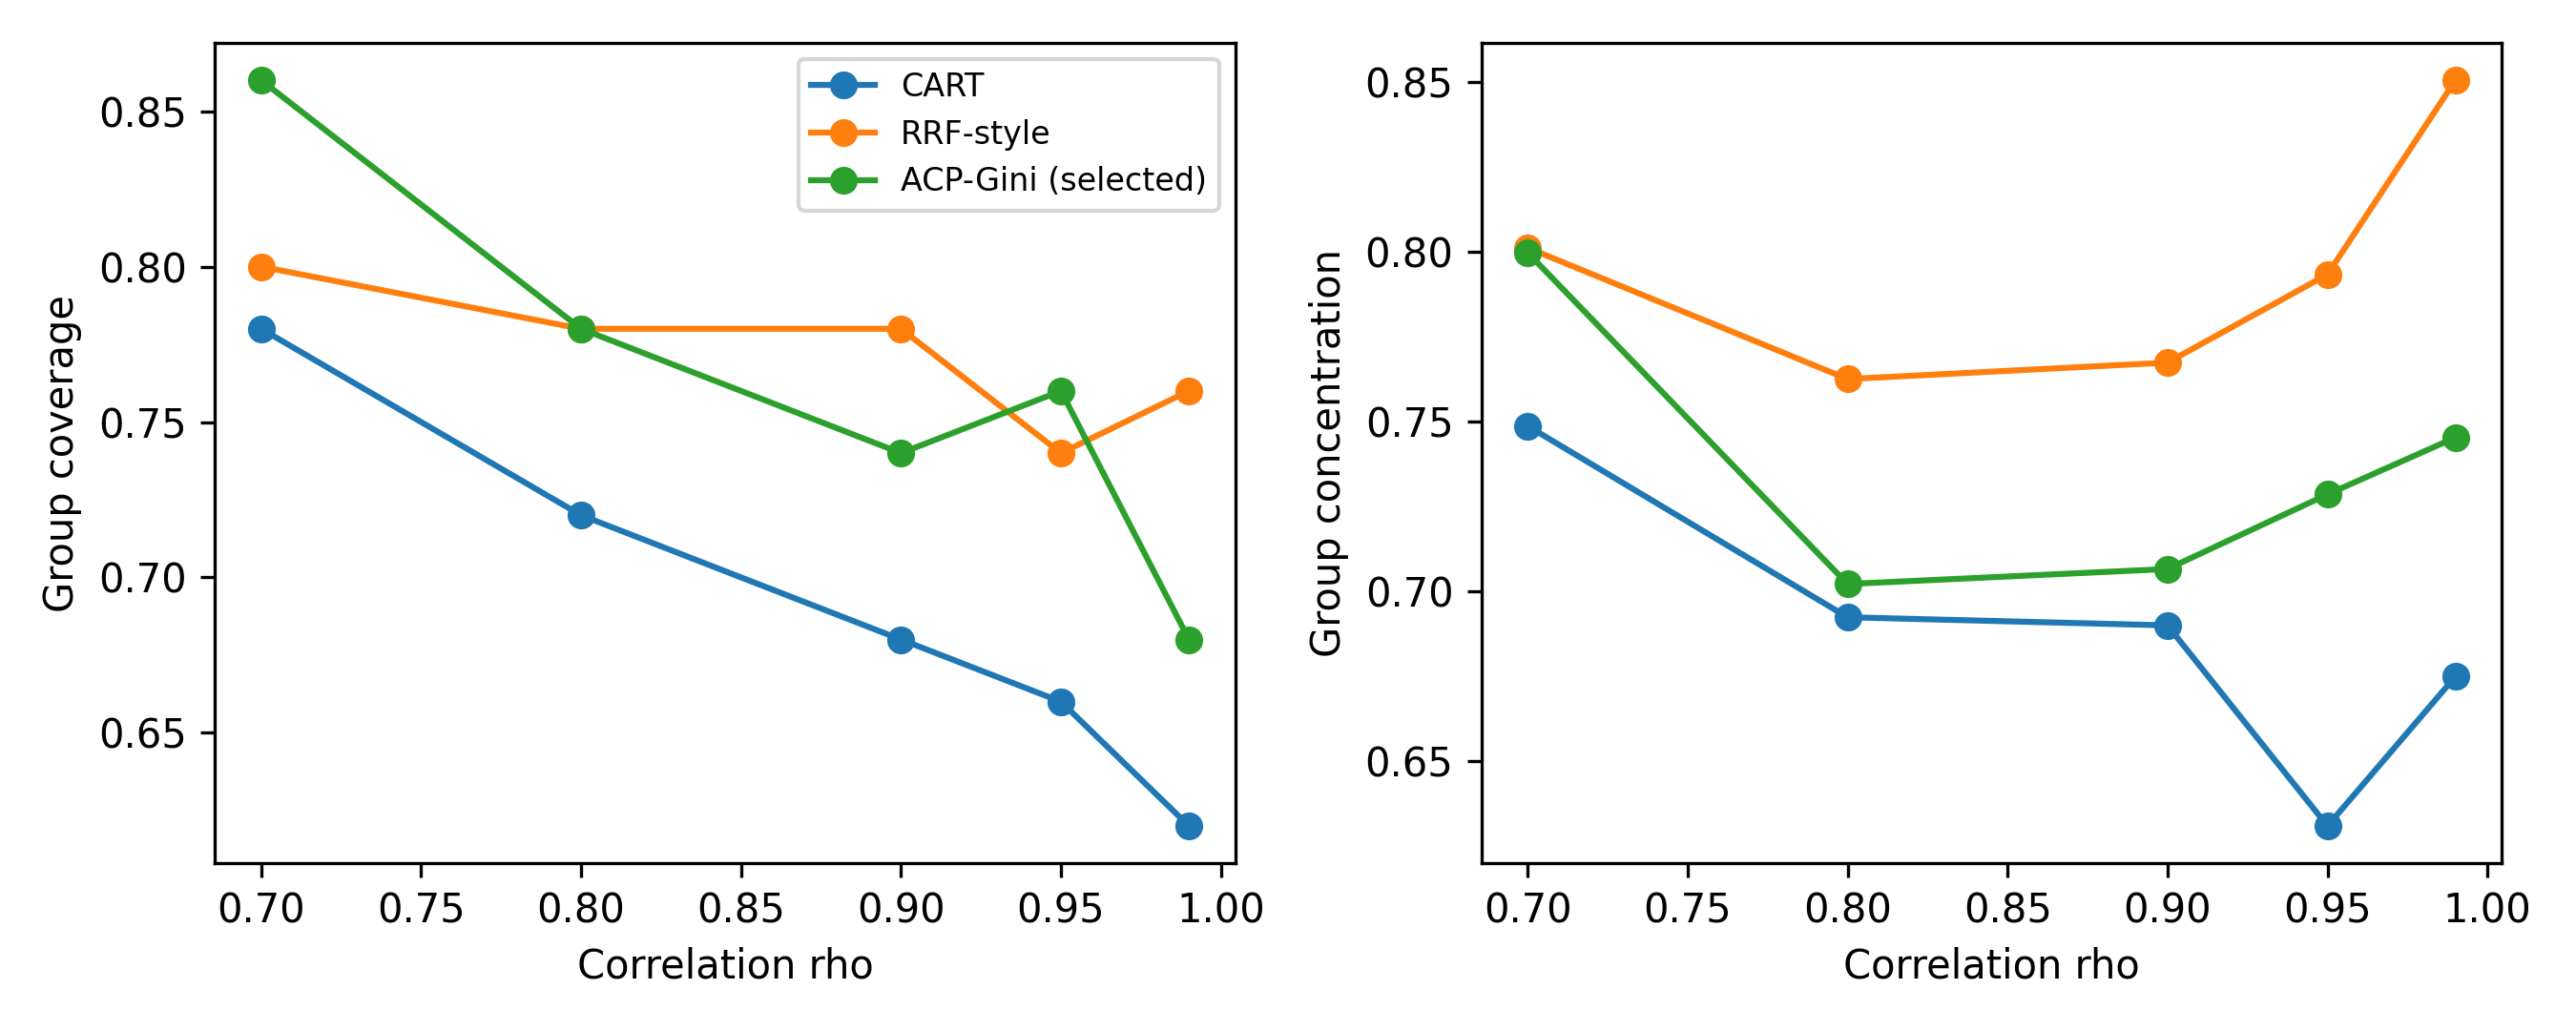
\includegraphics[width=.62\textwidth]{fig2_synthetic.png}
\caption{Synthetic group coverage and concentration (mean of ten repeats). RRF-style attains high concentration by feature reuse; Fig.~\ref{fig:forest} and Table~\ref{tab:redundancy} test transfer to real data.}\label{fig:synthetic}
\end{figure}

\subsubsection{Predictive performance}
Selected parameters are in Table~\ref{tab:data}. Across the twelve data sets the mean accuracy was 0.843 for ACP-Gini and 0.844 for CART (Table~\ref{tab:methods}), and none of the twelve corrected tests was significant (Table~\ref{tab:inference}). A non-significant test is not evidence of equivalence, so Table~\ref{tab:noninf} gives the intervals. For the consensus $\alpha$ the lower 95\% limit of the accuracy change ranged from $-0.5$ (Landsat) to $-5.5$ percentage points (Parkinsons), supporting non-inferiority at a 6-point margin on every data set and at a 2-point margin on WDBC, Wine, Pima, Landsat and Ozone only. The nested variant, which tunes $\alpha$ inside each outer fold, is the less biased estimate: its mean accuracy was 0.840 and its lower limits ranged from $-0.6$ to $-5.0$ points on ten data sets and reached $-8.3$ on Sonar and $-9.0$ on Parkinsons. Losses of several points on small data sets are therefore not excluded; the supported claim is the absence of a detectable change, not equivalence.

\begin{table}[!htbp]\centering\caption{Accuracy change of ACP-Gini relative to CART (percentage points) with 95\% corrected-resampled intervals, for the consensus $\alpha$ and for $\alpha$ tuned inside each outer fold.}\label{tab:noninf}\scriptsize\begin{tabular}{lcc}
\toprule
Data set & Consensus $\alpha$ & Nested $\alpha$ \\
\midrule
WDBC & +0.06 [-1.66, +1.78] & -0.06 [-2.48, +2.37] \\
Diabetes & +0.23 [-3.17, +3.63] & -0.00 [-4.42, +4.42] \\
Sonar & -0.65 [-4.85, +3.55] & -2.24 [-8.32, +3.84] \\
Cultivar & -0.37 [-2.52, +1.79] & -0.18 [-2.55, +2.19] \\
Wine & -0.10 [-1.39, +1.19] & -0.05 [-1.31, +1.21] \\
Digits38 & +0.37 [-2.30, +3.05] & +0.47 [-2.22, +3.15] \\
Ionosphere & +0.09 [-2.77, +2.96] & -0.38 [-3.39, +2.63] \\
Pima & -0.43 [-1.49, +0.62] & +0.00 [-3.30, +3.30] \\
\bottomrule
\end{tabular}
\end{table}
\begin{table}[!htbp]\centering\caption{Mean over the twelve data sets of the per-data-set fold means. Bold marks a proposed-method value that is better than every baseline; redundancy and path columns are lower-is-better. Group corr. is the group-level importance rank correlation, $R_w$ the bootstrap importance-weighted redundancy and Path $|r|$ the bootstrap path correlation.}\label{tab:methods}\tiny\setlength{\tabcolsep}{2pt}\begin{tabular}{lccccccc}
\toprule
Method & Acc. & F1 & AUC & $R_w$ & Path $|r|$ & Rank corr. & Group corr. \\
\midrule
CART & 0.844 & 0.807 & 0.855 & 0.342 & 0.314 & 0.370 & 0.528 \\
VIF+CART & 0.840 & 0.802 & 0.855 & 0.292 & 0.277 & 0.456 & 0.496 \\
Cluster+CART & 0.840 & 0.802 & 0.856 & 0.304 & 0.279 & 0.395 & 0.480 \\
RRF-style & 0.842 & 0.805 & 0.854 & 0.337 & 0.305 & 0.361 & 0.527 \\
ACP-Gini & 0.843 & 0.807 & 0.854 & 0.293 & \textbf{0.259} & 0.375 & 0.489 \\
ACP-Gini (nested) & 0.840 & 0.803 & 0.855 & \textbf{0.271} & \textbf{0.237} & 0.377 & 0.483 \\
\bottomrule
\end{tabular}
\end{table}

\subsubsection{Selected-set and path-level redundancy}
ACP-Gini lowered bootstrap importance-weighted redundancy in all twelve data sets (sign test $p=0.0005$; Fig.~\ref{fig:forest}a, Table~\ref{tab:inference}). The relative reduction had a median of 12.5\% and ranged from 0.9\% on Pima to 32.3\% on Ozone, every Holm-adjusted $p$ was at most 0.0013, and on the four strongly collinear sets it was 12.1\% (WDBC), 25.9\% (Parkinsons), 6.6\% (Landsat) and 32.3\% (Ozone). The same held for single paths. Mean path correlation fell in all twelve data sets (Holm $p<0.001$), and the share of leaf samples reached through a path with a pair of $|r|>0.7$ fell from 86.2\% to 75.8\% on WDBC, from 88.2\% to 49.4\% on Ozone, from 29.0\% to 4.9\% on Parkinsons and from 11.7\% to 0.02\% on Wine; on Landsat, where almost every path holds such a pair, it stayed near 100\%. Pima, with no strongly correlated pairs, changed by 0.9\%, detectable but practically negligible. With $\alpha$ tuned inside each fold the reductions were similar or larger (mean $R_w$ 0.271 against 0.293 for the consensus value, Table~\ref{tab:methods}), and ten of the twelve remained significant after Holm adjustment (WDBC $p=0.079$, Landsat 0.094).

Because the penalty uses the same Pearson matrix as $R_w$, a reduction in $R_w$ alone could be largely mechanical. We therefore recomputed $R_w$ on the single fitted trees with Spearman $|\rho|$ and with normalized mutual information (\texttt{results/review\_checks.csv}). ACP-Gini lowered both in all twelve data sets (mean 0.362 to 0.321 with Spearman and 0.154 to 0.141 with mutual information); the mutual-information reductions were small (0.9\% to 2.8\%) on seven data sets and larger on Ozone (50.0\%), Wine (26.8\%), WDBC (16.0\%), Musk (8.0\%) and Parkinsons (6.9\%).

\begin{figure}[!htbp]
\centering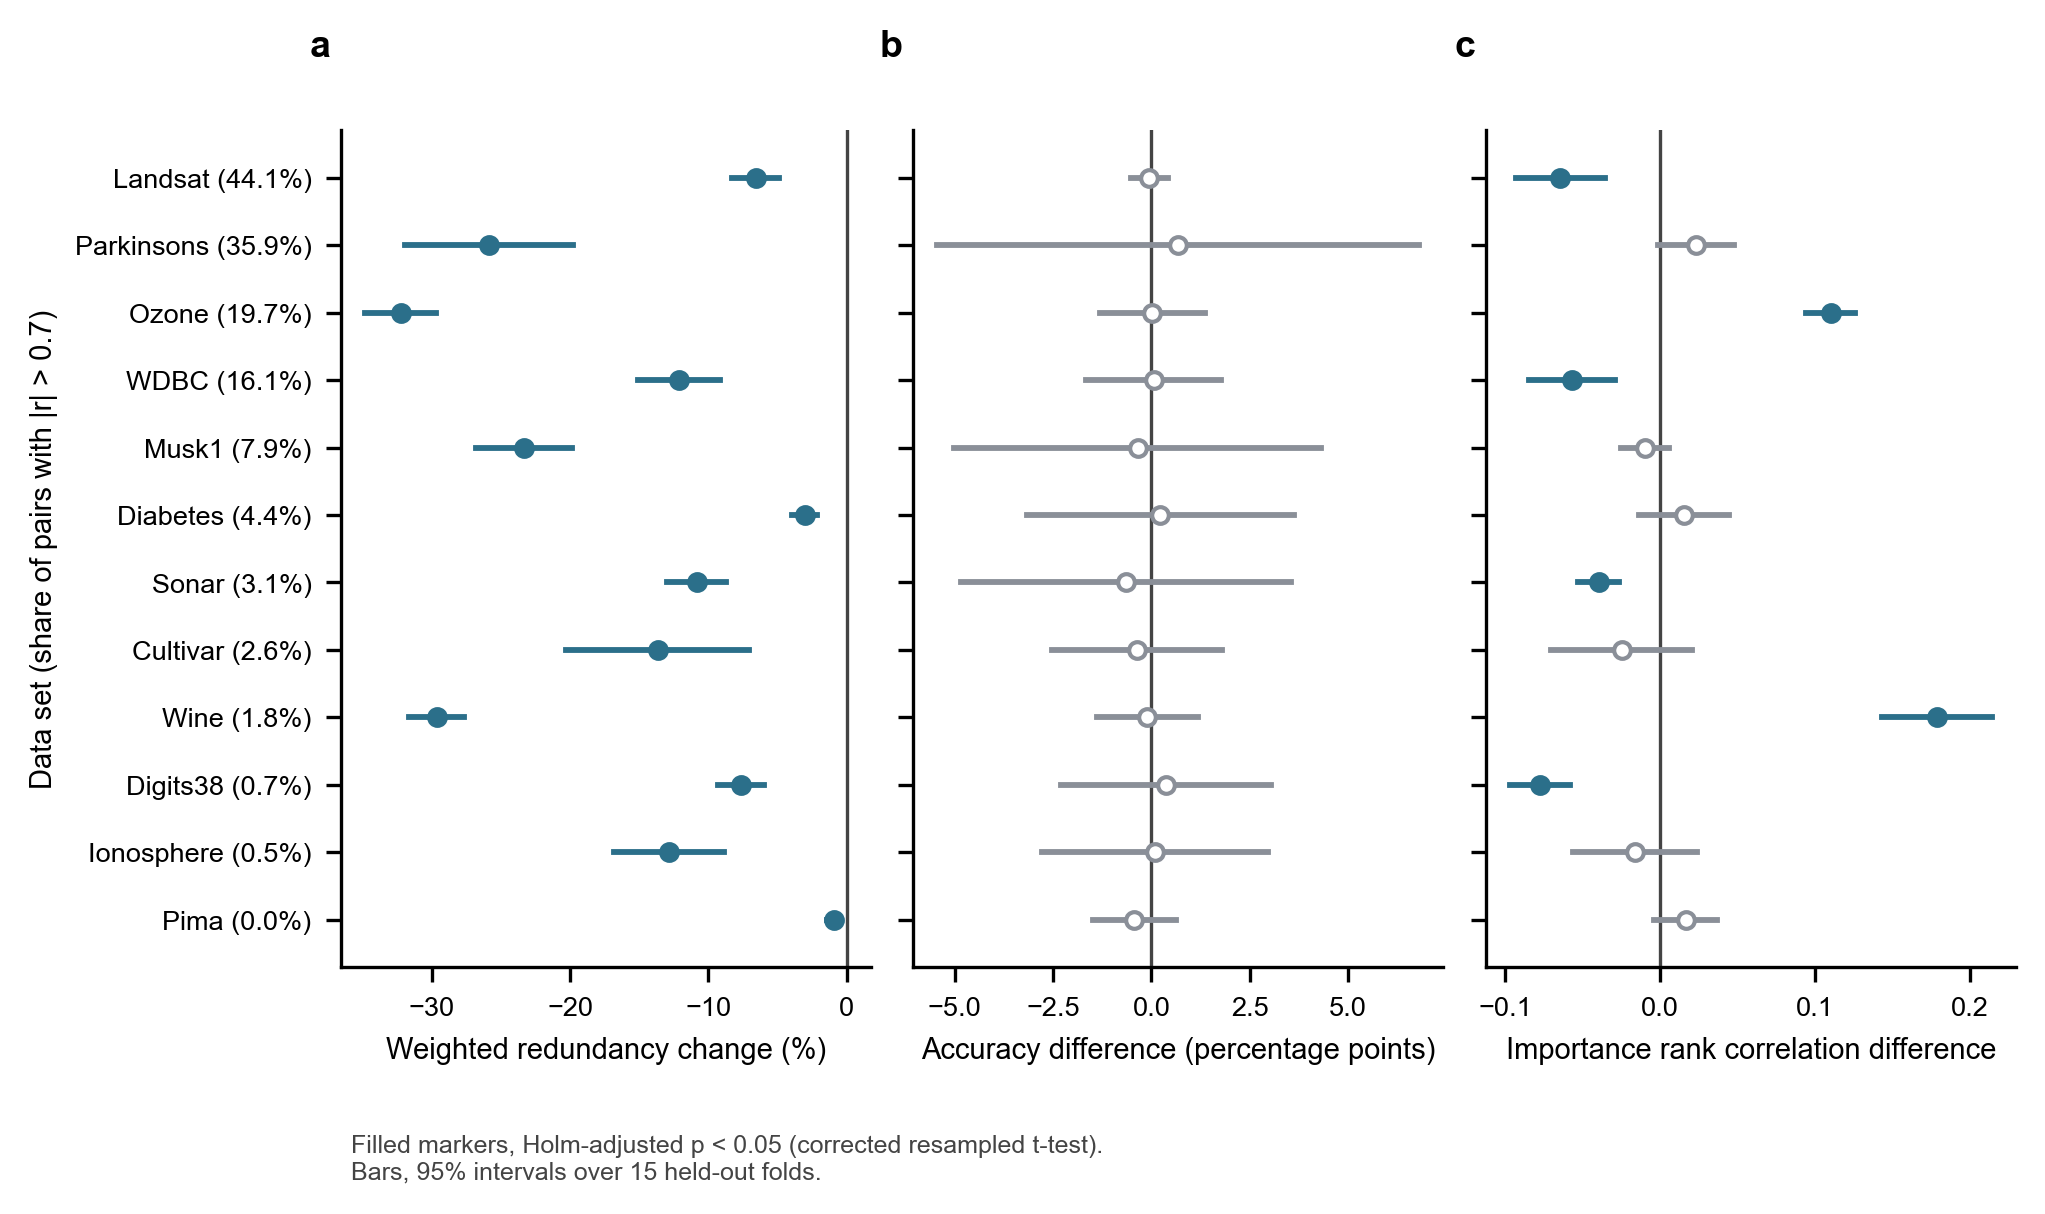
\includegraphics[width=.8\textwidth]{fig7_forest.png}
\caption{ACP-Gini minus CART per data set, ordered by the share of feature pairs with $|r|>0.7$: (a) relative change in bootstrap importance-weighted redundancy, (b) accuracy change, (c) change in importance rank correlation. Intervals are 95\% corrected-resampled-$t$ intervals over 15 folds; filled markers have Holm-adjusted $p<0.05$.}\label{fig:forest}
\end{figure}
\begin{table*}[!tbp]\centering\caption{ACP-Gini minus CART per data set with 95\% corrected-resampled intervals and Holm-adjusted $p$-values (pp, percentage points). Bold marks a significant change in favour of ACP-Gini (Holm $p<0.05$).}\label{tab:inference}\tiny\setlength{\tabcolsep}{2pt}\begin{tabular}{lccccc}
\toprule
Data set & Redundancy change (\%) [95\% CI] & Holm $p$ & Accuracy change (pp) [95\% CI] & Rank-corr. change [95\% CI] & Holm $p$ \\
\midrule
Landsat & \textbf{-6.6 [-8.3, -4.9]} & \textbf{$<$0.001} & -0.05 [-0.52, 0.41] & -0.064 [-0.093, -0.036] & 0.002 \\
Parkinsons & \textbf{-25.9 [-31.9, -19.8]} & \textbf{$<$0.001} & 0.68 [-5.45, 6.81] & +0.023 [-0.002, +0.048] & 0.384 \\
Ozone & \textbf{-32.3 [-34.8, -29.7]} & \textbf{$<$0.001} & 0.03 [-1.30, 1.35] & \textbf{+0.110 [+0.094, +0.126]} & \textbf{$<$0.001} \\
WDBC & \textbf{-12.1 [-15.1, -9.2]} & \textbf{$<$0.001} & 0.06 [-1.66, 1.78] & -0.057 [-0.085, -0.029] & 0.005 \\
Musk1 & \textbf{-23.3 [-26.8, -19.9]} & \textbf{$<$0.001} & -0.35 [-5.02, 4.32] & -0.010 [-0.025, +0.006] & 0.803 \\
Diabetes & \textbf{-3.0 [-3.9, -2.1]} & \textbf{$<$0.001} & 0.23 [-3.17, 3.63] & +0.015 [-0.014, +0.044] & 0.803 \\
Sonar & \textbf{-10.8 [-13.0, -8.7]} & \textbf{$<$0.001} & -0.65 [-4.85, 3.55] & -0.040 [-0.053, -0.026] & $<$0.001 \\
Cultivar & \textbf{-13.7 [-20.3, -7.1]} & \textbf{0.001} & -0.37 [-2.52, 1.79] & -0.025 [-0.070, +0.021] & 0.803 \\
Wine & \textbf{-29.6 [-31.6, -27.7]} & \textbf{$<$0.001} & -0.10 [-1.39, 1.19] & \textbf{+0.179 [+0.143, +0.214]} & \textbf{$<$0.001} \\
Digits38 & \textbf{-7.6 [-9.3, -6.0]} & \textbf{$<$0.001} & 0.37 [-2.30, 3.05] & -0.078 [-0.097, -0.058] & $<$0.001 \\
Ionosphere & \textbf{-12.9 [-16.8, -8.9]} & \textbf{$<$0.001} & 0.09 [-2.77, 2.96] & -0.016 [-0.056, +0.024] & 0.803 \\
Pima & \textbf{-0.9 [-1.4, -0.4]} & \textbf{0.001} & -0.43 [-1.49, 0.62] & +0.017 [-0.004, +0.037] & 0.496 \\
\bottomrule
\end{tabular}
\end{table*}

The removed correlation mass sits on shared paths. On Wine, CART path pairs with $|r|\ge0.5$ were 5.0\% of pair mass (density with alcohol, free with total sulfur dioxide, residual sugar with density) and none remained under ACP-Gini; the share of pair mass with $|r|\ge0.7$ fell from 32.1\% to 24.7\% on WDBC, from 20.3\% to 6.6\% on Ozone and from 15.7\% to 7.4\% on Parkinsons (\texttt{results/path\_band\_mass.csv}, \texttt{results/path\_pairs\_high\_corr.csv}). Wine's selected $\alpha$ is the grid maximum (1.0); in the single-tree sweep its reduction was 5.8\% at $\alpha=0.2$ and 29.1\% at $\alpha=1.0$ (Fig.~\ref{fig:operating}), so most of that effect comes from the strongest penalty.

\subsubsection{Stability}\label{subsec:stability}
Stability did not improve uniformly. Importance rank correlation was significantly lower than CART's on WDBC ($-0.057$), Sonar ($-0.040$), Digits38 ($-0.078$) and Landsat ($-0.065$), significantly higher on Wine ($+0.179$) and Ozone ($+0.110$), and not significantly different on the other six (Fig.~\ref{fig:forest}c, Table~\ref{tab:inference}). Across data sets the top-five metric was lower in 6 of 12 and the rank correlation in 7 of 12, but the used-feature Jaccard was lower in 11 of 12 (sign test $p=0.006$; \texttt{results/sign\_tests.csv}). The Wine gain is therefore metric-dependent, since its used-feature Jaccard fell from 0.986 to 0.898 while its rank correlation rose.

One could read the loss as harmless, a reshuffling among interchangeable members of one correlated block; then the rank correlation of group-aggregated importance would be unchanged. It was not. Groups come from the full-data correlations, and Pima has none with more than one member. On the other eleven data sets the group-level importance correlation was lower under ACP-Gini on ten, significantly so on WDBC (0.677 to 0.520), Sonar, Digits38 and Musk, and higher on Wine (0.752 to 0.850); the group-level Jaccard was lower in ten of twelve. We therefore report a real stability cost on most data sets with correlation structure. A plausible mechanism is that the penalty makes later choices depend on earlier ones, so a bootstrap perturbation of the root propagates through penalized children, but we have not tested this.


\subsubsection{Tree size and runtime}
Tree size changed little. The mean node count of ACP-Gini was within 3.6\% of CART's on every data set (24.2 against 24.7 on WDBC). Fit time at $\alpha=0.6$ was 0.98 to 1.56 times CART for the global scope and 1.02 to 1.37 times for the node-local scope, with mean fit times under 0.27 s on one machine, so the overhead is small.

\section{Discussion}
ACP-Gini lowered redundancy without a significant accuracy change, at the price of lower stability on most data sets with correlation structure. The subsections below examine the components, the errors, the baselines and recent work, and the uses and limits.

\subsection{Ablation Study and Component Analysis}
\subsubsection{Penalty strength, depth cap and correlation estimator}
Figure~\ref{fig:operating} shows how $\alpha$ moves the three costs (15 folds, 20 bootstrap refits per fold and $\alpha$). Averaged over data sets, raising $\alpha$ from 0.2 to 1.0 lowered importance-weighted redundancy by 9.1\% to 32.6\% and accuracy by 0.08 to 0.96 points. The rank-correlation change was about $-0.02$ at $\alpha=0.2$ and zero on average at $\alpha\ge0.8$, but its sign varies by data set (it fell in 8 of 12 data sets at $\alpha=0.2$ and in 6 at $\alpha=1$). On WDBC (single-tree sweep), $\alpha=0.6$ cut redundancy by 38.5\% at an accuracy change of $-0.2$ points and $\alpha=1.0$ by 57.8\% at $-1.3$ points; at $\alpha=1$ the accuracy cost reached 4.0 points on Sonar and 2.4 on Parkinsons. A depth cap of 3, 4, 6, 8 or 10 left the sign of the reduction unchanged in every data set except Pima at depth 3, with accuracy changes within 1.6 points (\texttt{results/depth\_sensitivity.csv}).

At the selected $\alpha$ (single fitted trees, \texttt{results/ablation\_full.csv}), the default (Pearson, product, global) gave the largest redundancy reduction (13.1\%), ahead of Spearman correlation (11.9\%), min (11.3\%) and mean (9.4\%) aggregation and the node-local scope (9.6\%, which also cost the most accuracy, 0.5 points against at most 0.2 for the others). Product aggregation with global Pearson correlation is therefore the simplest effective default.

\begin{figure}[!htbp]
\centering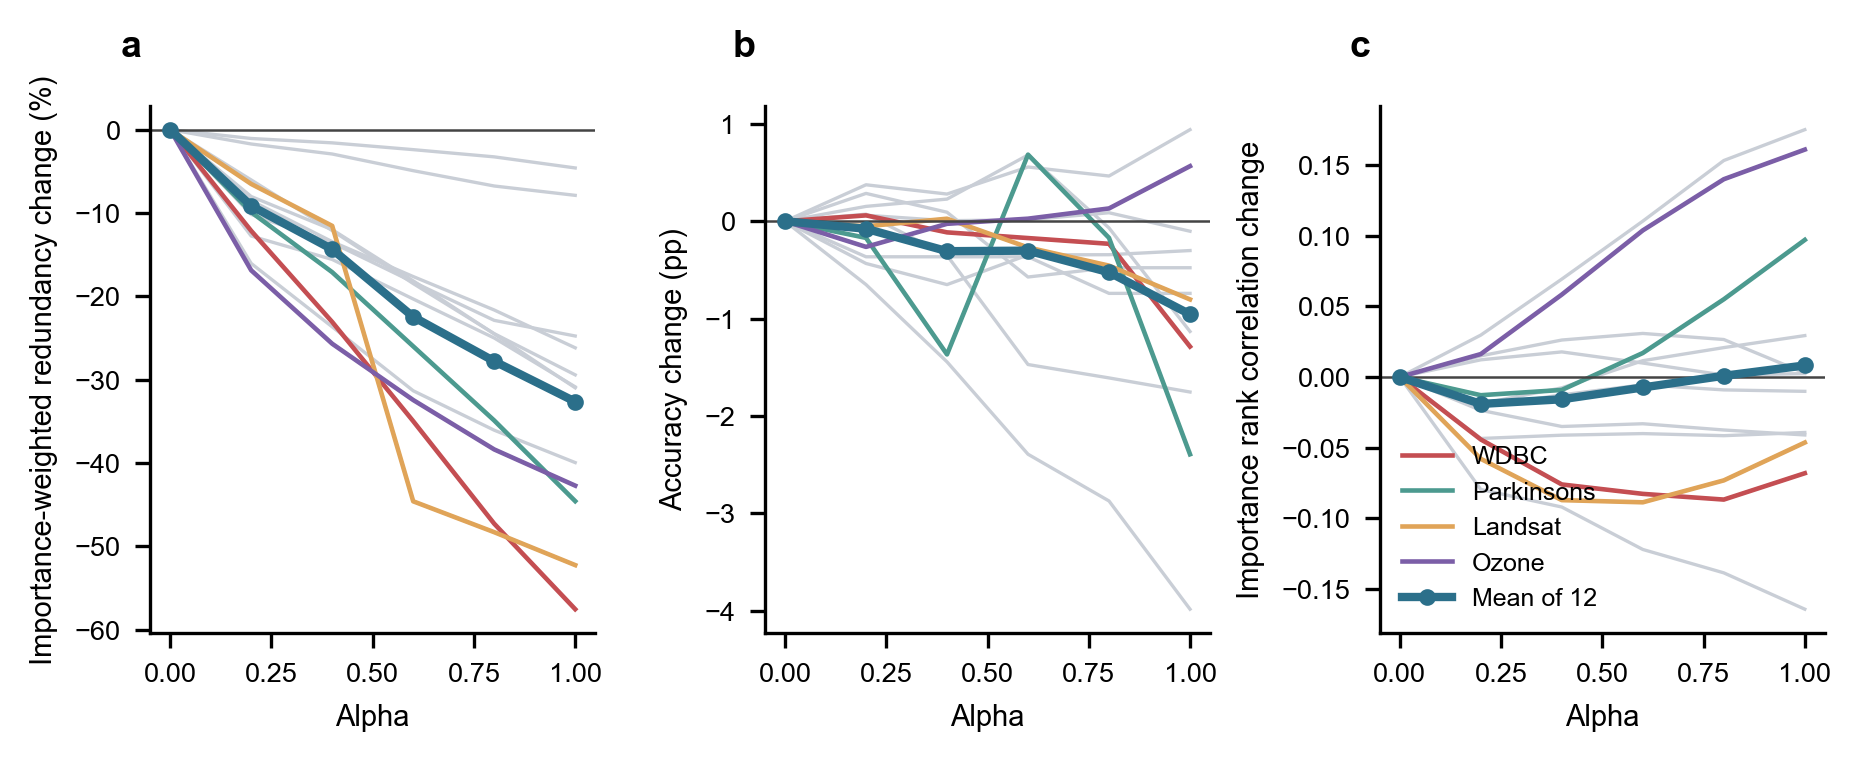
\includegraphics[width=.88\textwidth]{fig10_operating_curves.png}
\caption{Effect of $\alpha$ relative to CART ($\alpha=0$) on (a) bootstrap importance-weighted redundancy, (b) accuracy and (c) importance rank correlation. Grey lines are the other eight data sets; coloured lines are the four strongly collinear data sets; the thick line is the mean of the twelve data sets.}\label{fig:operating}
\end{figure}

\subsubsection{Does path-local scope matter, and how do tuned filters compare?}\label{subsec:scope}
Two checks address the weakest points of the comparison. First, we replaced the path-local penalty by one over every feature used anywhere so far in the tree. It gave slightly lower average redundancy (0.290 against 0.300 with Pearson, 0.313 against 0.321 with Spearman, 0.137 against 0.141 with mutual information) at the same accuracy (0.844 against 0.843), so on these data the path-local scope is not shown to be necessary and the active ingredient is the correlation-aware discount. Second, we swept the filter thresholds on the same folds. At threshold 10, VIF+CART matched ACP-Gini on average redundancy (0.301) keeping 25.4 of 43.0 features; at threshold 5 it was lower (0.275) with 20.4 kept and 0.4 points less accuracy; Cluster+CART at $|r|\ge0.5$ reached 0.277 with 15.5 kept. Tuned or swept, the filters are competitive on redundancy and differ mainly in discarding features (\texttt{results/review\_checks.csv}).

\subsubsection{Controlled scenarios with known structure}\label{subsec:scenarios}
To test when the path-local scope and feature availability matter, we built two scenarios with known structure (Table~\ref{tab:scenarios}; 30 and 50 replicates, 70/30 splits, penalty variants at $\alpha=1$). In S1 five latent signals have three noisy copies at correlation $\rho$, as in Section~\ref{subsec:setup}. At $\rho=0.9$ the group concentration was 0.669 for CART, 0.711 for path-local ACP-Gini, 1.000 for the tree-global penalty and 0.973 for Cluster+CART, so the path-local penalty is the weakest suppressor of redundant copies; accuracy differed by less than 0.4 points except for VIF+CART (3.7 lower). In S2 a gate selects one of two regimes: feature $a$ reproduces a latent signal on the left and is noise on the right, while $b$ is a noisy copy of it on the left and the label-relevant feature on the right, so $a$ and $b$ are strongly correlated overall (0.68 and 0.77 with 70\% and 80\% of samples on the left) although $a$ is never used on the right path. The gate was chosen at the root in all runs at 70\% left and in 86\% at 80\%. In the right regime path-local ACP-Gini matched CART (0.912 against 0.911 at 70\% left, 0.907 against 0.908 at 80\%), whereas the tree-global penalty fell to 0.898 and 0.889 (paired differences of 1.4 and 1.7 points, $p<10^{-4}$) and Cluster+CART, which keeps one of $a$ and $b$, to 0.892 and 0.769. S2 was constructed and piloted to separate the variants; it shows that the path-local scope can matter, not how often such structure occurs.

\begin{table}[!htbp]\centering\caption{Controlled scenarios, mean over replicates. S1: group concentration and accuracy at $\rho=0.9$. S2: accuracy in the right regime with 70\% and 80\% of samples on the left, and overall accuracy at 80\%. Bold marks ACP-Gini where it is the best of all methods.}\label{tab:scenarios}\tiny\setlength{\tabcolsep}{2pt}\begin{tabular}{lccccc}
\toprule
Method & S1 conc. & S1 acc. & S2 right (0.7) & S2 right (0.8) & S2 acc. (0.8) \\
\midrule
CART & 0.669 & 0.795 & 0.911 & 0.908 & 0.924 \\
ACP-Gini (path-local) & 0.711 & \textbf{0.796} & \textbf{0.912} & 0.907 & \textbf{0.924} \\
Correlation penalty, tree-global & 1.000 & 0.793 & 0.898 & 0.889 & 0.920 \\
ACP-Gini (node-local scope) & 0.739 & 0.796 & 0.910 & 0.907 & 0.924 \\
VIF+CART & 0.638 & 0.758 & 0.911 & 0.908 & 0.924 \\
Cluster+CART & 0.973 & 0.793 & 0.892 & 0.769 & 0.897 \\
\bottomrule
\end{tabular}
\end{table}

\subsection{Analysis of Model Errors and Case Study}
On WDBC, CART and ACP-Gini disagreed on 53 of 1707 test predictions across the 15 folds (3.1\%). ACP-Gini was right on 27 of these and CART on 26, and 16 lay near the $[0.4,0.6]$ probability boundary, so the tree change does not systematically favour either model.

Table~\ref{tab:casestudy} traces the mechanism at the right child of the WDBC root, whose path ancestor is worst concave points (Fig.~\ref{fig:trees}). CART picks mean texture on raw gain. Its correlation of 0.353 with the ancestor gives a penalty factor of 0.929. Texture error has slightly lower raw gain but a correlation of 0.112 with the ancestor, so its factor is 0.978, and ACP-Gini selects it; by P4 the ranking reverses at $\alpha^*=0.148$, below the selected $\alpha=0.2$. Mean texture is moderately, not strongly, correlated with the ancestor, which is the regime where the penalty reorders near-ties without suppressing informative splits.

\begin{figure}[!htbp]
\centering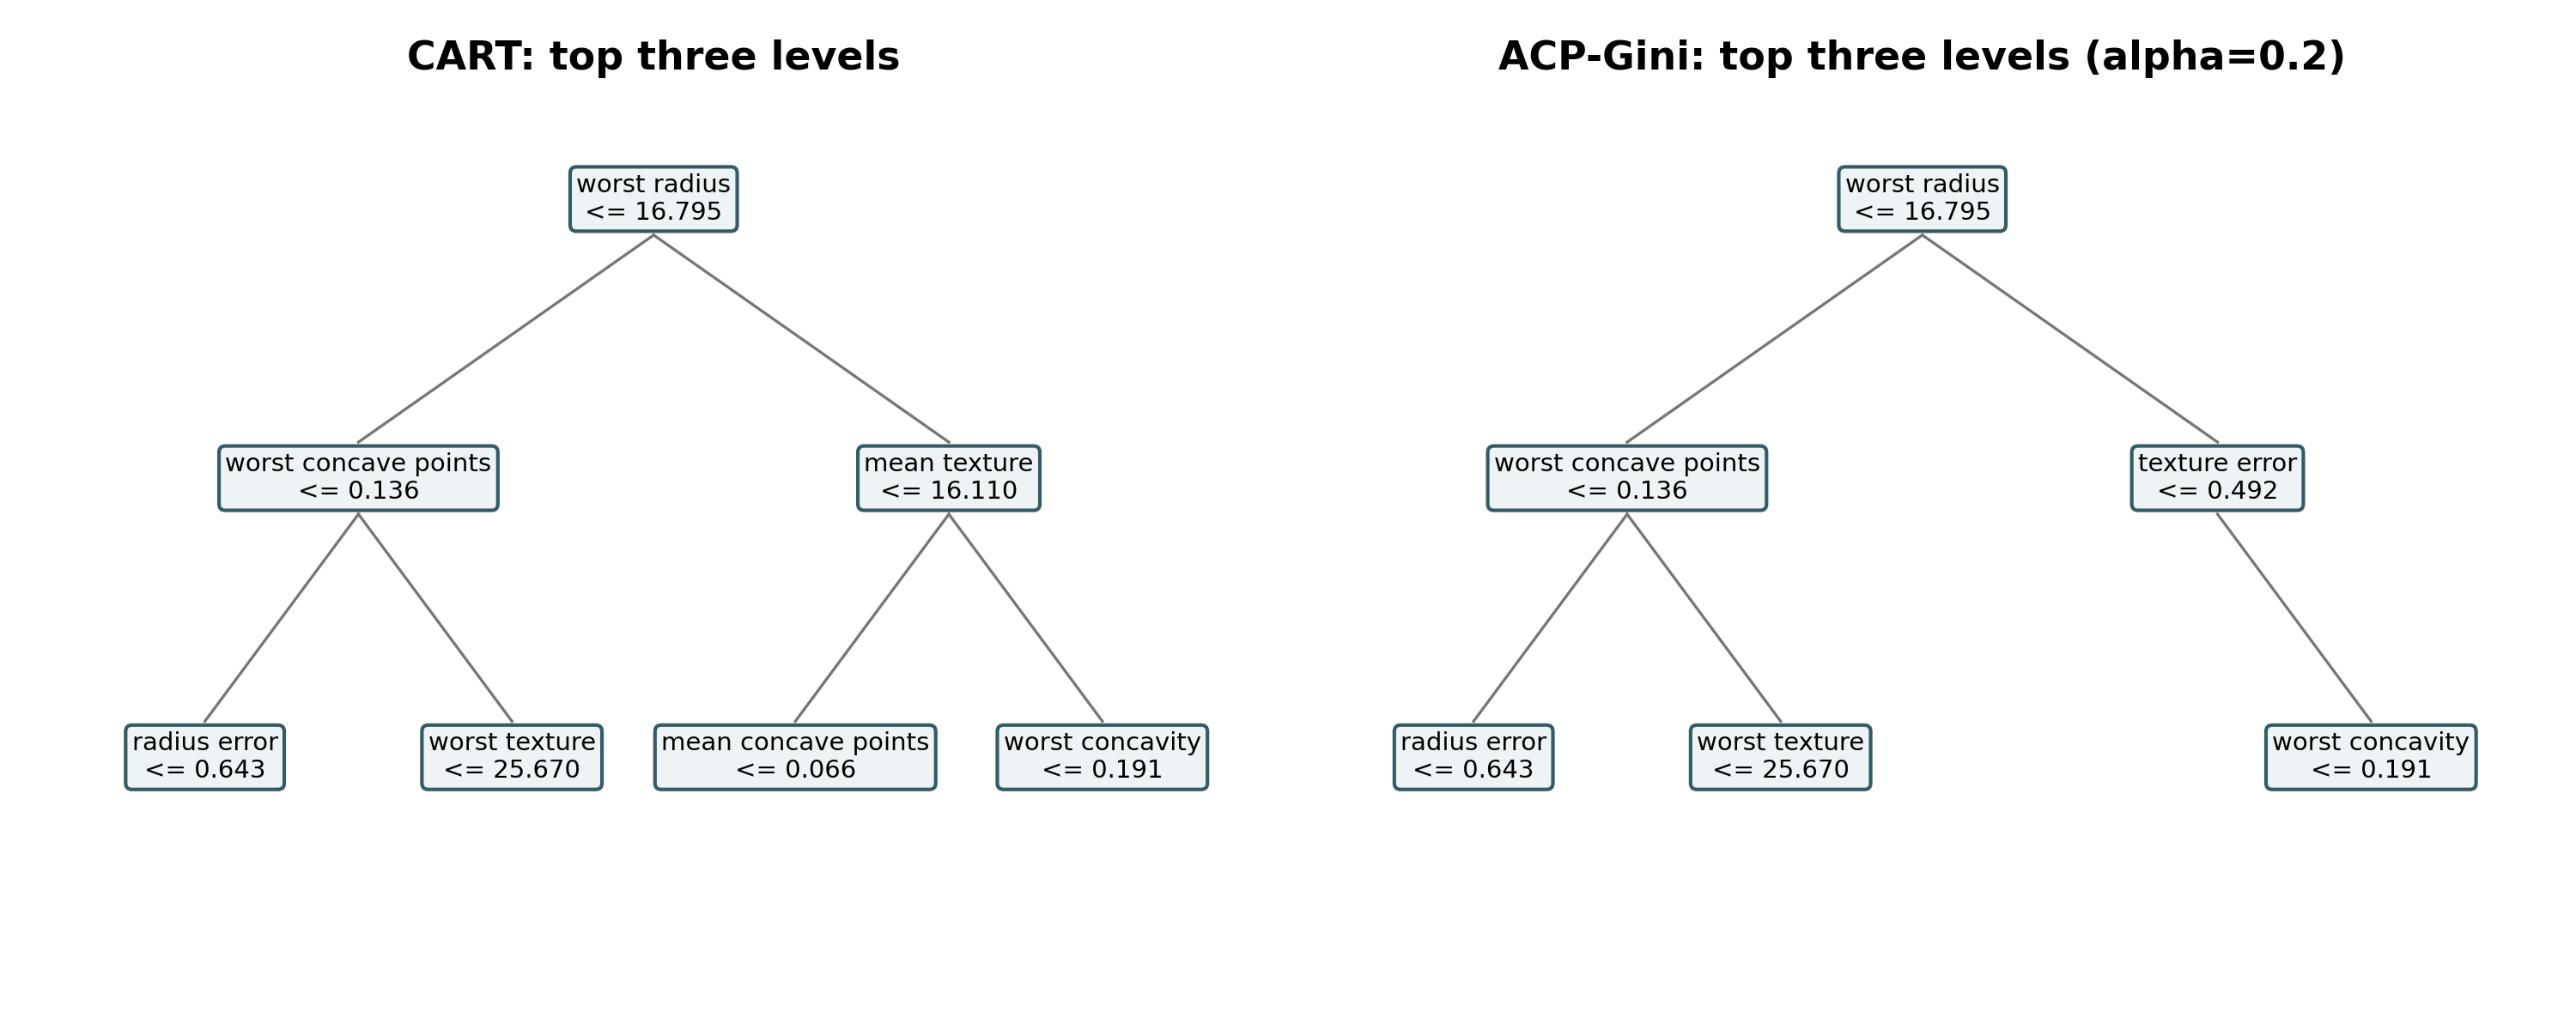
\includegraphics[width=.8\textwidth]{fig5_tree_comparison.png}
\caption{Top three levels of full-data WDBC trees at the selected $\alpha=0.2$.}\label{fig:trees}
\end{figure}
\begin{table}[h]\centering\caption{Candidate split evaluations at the WDBC root's right child (selected $\alpha=0.2$); the candidate that ACP-Gini selects is in bold.}\label{tab:casestudy}\tiny\setlength{\tabcolsep}{2pt}\begin{tabular}{lrrrrrr}
\toprule
Feature & Raw Gain & Corr with Root & Penalty & ACP Score & CART Rank & ACP Rank \\
\midrule
mean texture & 0.0437 & 0.3526 & 0.9295 & 0.0406 & 1 & 2 \\
worst texture & 0.0437 & 0.3599 & 0.9280 & 0.0405 & 2 & 3 \\
texture error & 0.0421 & 0.1117 & 0.9777 & 0.0412 & 3 & 1 \\
mean concavity & 0.0412 & 0.6882 & 0.8624 & 0.0355 & 4 & 4 \\
worst concavity & 0.0372 & 0.5740 & 0.8852 & 0.0330 & 5 & 5 \\
\bottomrule
\end{tabular}
\end{table}


\subsection{Comparison with Baselines and State-of-the-Art Approaches}
Table~\ref{tab:redundancy} compares importance-weighted redundancy across methods and Table~\ref{tab:vsfilters} tests ACP-Gini against each baseline. ACP-Gini had the lowest point estimate on nine of twelve data sets (tying VIF+CART on Sonar). Against VIF+CART it was significantly lower on seven, indistinguishable on Sonar, Diabetes and Musk, and significantly higher on WDBC and Landsat; against Cluster+CART it was significantly lower on ten and higher on Landsat; against RRF-style it was significantly lower on all twelve. The four strongly collinear data sets split evenly against VIF+CART: ACP-Gini was lower on Parkinsons (0.328 against 0.406) and Ozone (0.233 against 0.271), where VIF+CART dropped 9.9 of 22 and 32.6 of 72 features, and higher on WDBC (0.545 against 0.343) and Landsat (0.539 against 0.476), where it dropped 13.3 of 30 and 26.5 of 36. Averaged over data sets, VIF+CART (0.292) equalled the consensus ACP-Gini (0.293) and was above the nested ACP-Gini (0.271). RRF-style and CART were nearly identical on real data (0.337 against 0.342), so the high synthetic concentration of RRF-style does not transfer. Mean accuracy was within 0.4 points of CART for every method (Table~\ref{tab:methods}).

The filters used fixed conventional thresholds while $\alpha$ was tuned, so Section~\ref{subsec:scope} sweeps their thresholds. VIF+CART was also the most stable method on average (rank correlation 0.456 against 0.370 for CART and 0.375 for ACP-Gini) and above ACP-Gini on six data sets (Holm $p<0.05$), whereas ACP-Gini was higher only on Wine; this metric counts dropped features as unused, which favours a method that removes features.

\begin{table}[!htbp]\centering\caption{Bootstrap importance-weighted redundancy $R_w$ by method (lower is better). Bold marks ACP-Gini where it has the lowest value.}\label{tab:redundancy}\scriptsize\setlength{\tabcolsep}{3pt}\begin{tabular}{lccccc}
\toprule
Data set & CART & VIF+CART & Cluster+CART & RRF-style & ACP-Gini \\
\midrule
Landsat & 0.577 & 0.476 & 0.433 & 0.557 & 0.539 \\
Parkinsons & 0.443 & 0.406 & 0.395 & 0.429 & \textbf{0.328} \\
Ozone & 0.345 & 0.271 & 0.240 & 0.340 & \textbf{0.233} \\
WDBC & 0.621 & 0.343 & 0.526 & 0.603 & 0.545 \\
Musk1 & 0.191 & 0.135 & 0.162 & 0.182 & 0.147 \\
Diabetes & 0.352 & 0.344 & 0.357 & 0.353 & \textbf{0.341} \\
Sonar & 0.218 & 0.195 & 0.207 & 0.216 & \textbf{0.195} \\
Cultivar & 0.453 & 0.450 & 0.452 & 0.451 & \textbf{0.391} \\
Wine & 0.183 & 0.169 & 0.167 & 0.181 & \textbf{0.128} \\
Digits38 & 0.375 & 0.366 & 0.369 & 0.378 & \textbf{0.346} \\
Ionosphere & 0.168 & 0.167 & 0.166 & 0.166 & \textbf{0.146} \\
Pima & 0.180 & 0.180 & 0.180 & 0.180 & \textbf{0.178} \\
\bottomrule
\end{tabular}
\end{table}
\begin{table*}[!tbp]\centering\caption{ACP-Gini minus each baseline in bootstrap $R_w$, with 95\% corrected-resampled intervals and Holm-adjusted $p$ in parentheses (negative favours ACP-Gini). Bold marks a significantly lower $R_w$ for ACP-Gini.}\label{tab:vsfilters}\tiny\setlength{\tabcolsep}{2pt}\begin{tabular}{llll}
\toprule
Data set & vs VIF+CART & vs Cluster+CART & vs RRF-style \\
\midrule
Landsat & +0.064 [+0.056, +0.072] ($<$0.001) & +0.107 [+0.087, +0.126] ($<$0.001) & \textbf{-0.018 [-0.022, -0.013] ($<$0.001)} \\
Parkinsons & \textbf{-0.077 [-0.104, -0.051] ($<$0.001)} & \textbf{-0.066 [-0.087, -0.046] ($<$0.001)} & \textbf{-0.101 [-0.133, -0.069] ($<$0.001)} \\
Ozone & \textbf{-0.038 [-0.045, -0.031] ($<$0.001)} & \textbf{-0.007 [-0.013, -0.001] (0.050)} & \textbf{-0.107 [-0.115, -0.098] ($<$0.001)} \\
WDBC & +0.202 [+0.141, +0.263] ($<$0.001) & +0.019 [-0.014, +0.053] (0.230) & \textbf{-0.058 [-0.076, -0.040] ($<$0.001)} \\
Musk1 & +0.011 [+0.002, +0.020] (0.057) & \textbf{-0.015 [-0.021, -0.010] ($<$0.001)} & \textbf{-0.036 [-0.041, -0.030] ($<$0.001)} \\
Diabetes & -0.003 [-0.007, +0.001] (0.240) & \textbf{-0.016 [-0.021, -0.011] ($<$0.001)} & \textbf{-0.012 [-0.014, -0.010] ($<$0.001)} \\
Sonar & -0.000 [-0.008, +0.008] (0.961) & \textbf{-0.012 [-0.020, -0.005] (0.010)} & \textbf{-0.021 [-0.028, -0.015] ($<$0.001)} \\
Cultivar & \textbf{-0.059 [-0.092, -0.025] (0.008)} & \textbf{-0.061 [-0.086, -0.035] ($<$0.001)} & \textbf{-0.061 [-0.091, -0.030] (0.002)} \\
Wine & \textbf{-0.041 [-0.044, -0.038] ($<$0.001)} & \textbf{-0.038 [-0.043, -0.033] ($<$0.001)} & \textbf{-0.053 [-0.057, -0.049] ($<$0.001)} \\
Digits38 & \textbf{-0.020 [-0.025, -0.015] ($<$0.001)} & \textbf{-0.023 [-0.032, -0.014] ($<$0.001)} & \textbf{-0.032 [-0.039, -0.025] ($<$0.001)} \\
Ionosphere & \textbf{-0.021 [-0.027, -0.015] ($<$0.001)} & \textbf{-0.019 [-0.026, -0.012] ($<$0.001)} & \textbf{-0.020 [-0.027, -0.014] ($<$0.001)} \\
Pima & \textbf{-0.002 [-0.003, -0.001] (0.007)} & \textbf{-0.002 [-0.003, -0.001] (0.005)} & \textbf{-0.001 [-0.002, -0.001] (0.005)} \\
\bottomrule
\end{tabular}
\end{table*}


Two findings narrow the claim against the baselines. On real data a tree-global penalty gave an equal or slightly larger average redundancy reduction than the path-local one, so those data do not show the path-local scope to matter; it matters in the controlled conditional scenario, where the tree-global penalty and Cluster+CART lose accuracy that path-local ACP-Gini keeps, and it costs redundancy suppression where no such structure exists (S1). Swept or tuned, the filters are competitive on real data: VIF at threshold 10 equals ACP-Gini on average, lower thresholds do better, and on WDBC and Landsat the filters beat the consensus ACP-Gini while on Parkinsons and Ozone ACP-Gini beat VIF+CART. What ACP-Gini offers over a filter is that no feature is removed, so a variable can still be used on a branch where it carries conditional information; we showed the benefit of that availability only in a constructed scenario, not on a real data set.

Our comparison with recent work is limited by scope. ACP-Gini targets a single readable tree, whereas the strongest tabular predictors are ensembles and tabular foundation models \cite{hollmann2025tabpfn,erickson2025tabarena}; we did not measure that accuracy gap, which any single interpretable tree shares. Optimal sparse and Rashomon-set methods \cite{zhang2023osrt,babbar2025split,arslan2025sorted,hsu2025rashomon} optimize or enumerate trees under global objectives, and trade-off studies include fairness \cite{jo2023fair}, whereas ACP-Gini is a greedy criterion; we did not benchmark against these solvers and claim no superiority. Their objectives omit predictor correlation, so the approaches are complementary, and a correlation-aware term inside an optimal-tree objective is a direction we have not tested.

\subsection{Interpretability Implications and Applications}
The reduction follows the correlation structure and the penalty strength rather than a fixed rate. It was largest on Ozone (32.3\%), Wine (29.6\%, at the grid maximum $\alpha=1$; 5.8\% at $\alpha=0.2$ in the single-tree sweep), Parkinsons (25.9\%) and Musk (23.3\%), and negligible on Pima. Landsat, the most collinear set, showed 6.6\% at its selected $\alpha=0.2$ and 52.2\% at $\alpha=1$, so on strongly collinear data the consensus value is conservative.

The stability result changes how the method should be presented. The penalty improved importance-rank stability on Wine and Ozone, lowered it on four data sets and lowered used-feature stability on eleven of twelve, and the group-level analysis shows the loss is not merely swapping within blocks. One untested reading is that interchangeable correlated predictors admit many near-equivalent trees, the multiplicity studied in Rashomon-set work \cite{arslan2025sorted,hsu2025rashomon}, and a path-dependent penalty chooses among them in a way that varies across bootstrap samples. For auditing one fitted tree this may be acceptable; where the identity of the top features must be reproducible across resamples it is not.

In practice, ACP-Gini suits settings in which a human reviews the rules of a single tree and the same evidence should not appear under several feature names, for example screening or risk scoring on tabular records. These uses are intended, not validated, because we ran no study of reviewers auditing trees.

\subsection{Research Limitations and Future Prospects}\label{subsec:limits}
The evidence has limits. All data sets are small to mid-sized, tabular and binary, and only four (WDBC, Parkinsons, Landsat and Ozone) are strongly collinear by the $|r|>0.7$ criterion, so statements about that regime rest on four data sets. Seven of the twelve data sets were added after the original five without pre-specification, and repeated measurements in Parkinsons and Musk can fall in different folds. The redundancy measures derive from the correlation matrix the penalty uses, and we ran no user study of audit quality. The main comparison does not match tuning, because $\alpha$ is tuned while the filter thresholds are fixed; the sweeps in Section~\ref{subsec:scope} report operating points, not a tuned protocol. The corrected resampled test, derived for test error, is applied to bootstrap-derived metrics as an approximation, and the Holm adjustment covers data sets within each metric only. ACP-Gini is a greedy heuristic without a stability guarantee, linear correlation cannot separate redundancy from useful nonlinear interaction, and a very strong penalty ($\alpha=1$) can expose weak splits on noise features.


Future work should test non-linear association measures, regression trees, ensembles, a stability objective inside the criterion, larger collinear benchmarks and a controlled study of reviewers auditing trees.

\section{Conclusion}
We set out to reduce the correlation redundancy that greedy decision trees accumulate under multicollinearity while keeping a single readable tree. ACP-Gini, a Gini split score discounted by each candidate's correlation with the features already used on its path, reduces to CART at $\alpha=0$. It lowered importance-weighted redundancy and mean path correlation in all twelve data sets (median redundancy reduction 12.5\%), also under Spearman and mutual-information measures, with no detectable accuracy change, although losses of several points on small data sets are not excluded. It did not improve stability in general: importance-rank stability fell significantly on four data sets and rose on two. Against VIF pruning on the four strongly collinear sets it won on two and lost on two, and on real data a tree-global penalty and tuned filters were competitive on redundancy; only in a designed conditional scenario did the path-local penalty preserve accuracy that they lost. The contribution is thus a correlation-aware split discount that keeps every feature available, with a controllable trade-off among redundancy, accuracy and stability, supported by twelve binary data sets (four strongly collinear) and redundancy measures rather than a user study of audit quality.

\setlength{\bibsep}{2pt}\renewcommand{\bibfont}{\footnotesize}
\bibliography{references}
\end{document}
